\documentclass[conference]{IEEEtran}
\usepackage[utf8]{inputenc}
\usepackage{booktabs}
\usepackage{graphicx}
\usepackage[hidelinks]{hyperref}
\usepackage{amsmath}
\usepackage{amssymb}
\usepackage{bbm}
\usepackage{float}

% --- FIXES FOR LAST PAGE ---
\usepackage{xurl}      % Allows the long GitHub URL to break nicely
\usepackage{flushend}  % Automatically balances the columns on the last page
% ---------------------------

\graphicspath{{../plots/}}

\title{SemEval-2026 Task 4: Hybrid Architecture for\\Cost-Efficient Narrative Similarity}

\author{
\IEEEauthorblockN{Muhammad Musaab-Ul-Haq (501739), Ahmed Hassan Raza (511263),\\Abdul Mueed (501166), Usman Amjad (516261)}
\IEEEauthorblockA{CS-272: Artificial Intelligence\\
National University of Sciences and Technology (NUST)}
}

\begin{document}
\maketitle

\begin{abstract}
We present a hybrid architecture for narrative similarity detection that achieves 96.8\% of optimal LLM accuracy while reducing inference costs by 27\%. Building on our Assignment 2 baselines, we explore two improvements: (1) multi-task learning to enhance embedding representations, and (2) a confidence-based routing system that combines fast embedding predictions with LLM reasoning for uncertain cases. The proposed hybrid system achieves 69.5\% accuracy on the development set, compared to 71.8\% for pure LLM inference, while requiring only 73\% of the computational cost. Systematic threshold optimization identifies the optimal confidence boundary for routing decisions.
\end{abstract}

\section{Introduction}

Narrative similarity detection---determining which of two candidate stories is more similar to an anchor story---presents unique challenges beyond standard semantic similarity. As established in Assignment 1, narratives contain complex temporal structures, thematic arcs, and abstract concepts that resist simple lexical matching (52.5\% accuracy with TF-IDF).

Our Assignment 2 experiments identified Chain-of-Thought (CoT) LLM reasoning as the most effective approach, achieving 71.8\% accuracy. However, LLM inference incurs significant computational costs.

\subsection{Contributions}
\begin{enumerate}
    \item \textbf{Multi-task Learning:} We investigate joint training with ranking and classification objectives to improve embedding representations.
    \item \textbf{Hybrid Architecture:} We propose a confidence-based routing system using fast embeddings for high-confidence predictions and LLM calls for uncertain cases.
    \item \textbf{Threshold Optimization:} We systematically analyze accuracy-cost trade-offs across confidence thresholds.
\end{enumerate}

\section{Proposed Method}

\subsection{Data Augmentation}

To address error patterns identified in Assignment 1, we generated 500 additional training samples targeting stories with misleading lexical overlap, narratives requiring abstract reasoning, and cases where setting vocabulary differs but plot structures align. These were combined with the original 2,400 synthetic triplets.

\subsection{Multi-task Learning Architecture}

We extended SentenceTransformer fine-tuning with dual training objectives:

\textbf{Head 1 - Semantic Ranking:} Using MultipleNegativesRankingLoss:
\begin{equation}
\mathcal{L}_{rank} = -\log \frac{e^{sim(a, p)/\tau}}{\sum_{n} e^{sim(a, n)/\tau}}
\end{equation}

\textbf{Head 2 - Binary Classification:} Using SoftmaxLoss for explicit similarity decisions. Training alternates batches between objectives, sharing base encoder weights.

\subsection{Hybrid Inference Architecture}

Our hybrid system operates in two stages (Figure~\ref{fig:architecture}):

\textbf{Stage 1 - Fast Embedding Prediction:}
Given triplet $(A, T_a, T_b)$, compute cosine similarities $s_a$, $s_b$ and confidence $= |s_a - s_b|$.

\textbf{Stage 2 - Routing Decision:}
\begin{equation}
\text{prediction} = 
\begin{cases}
\mathbbm{1}[s_a > s_b] & \text{if confidence} \geq \tau \\
\text{LLM}(A, T_a, T_b) & \text{otherwise}
\end{cases}
\end{equation}

\begin{figure}[t]
\centering
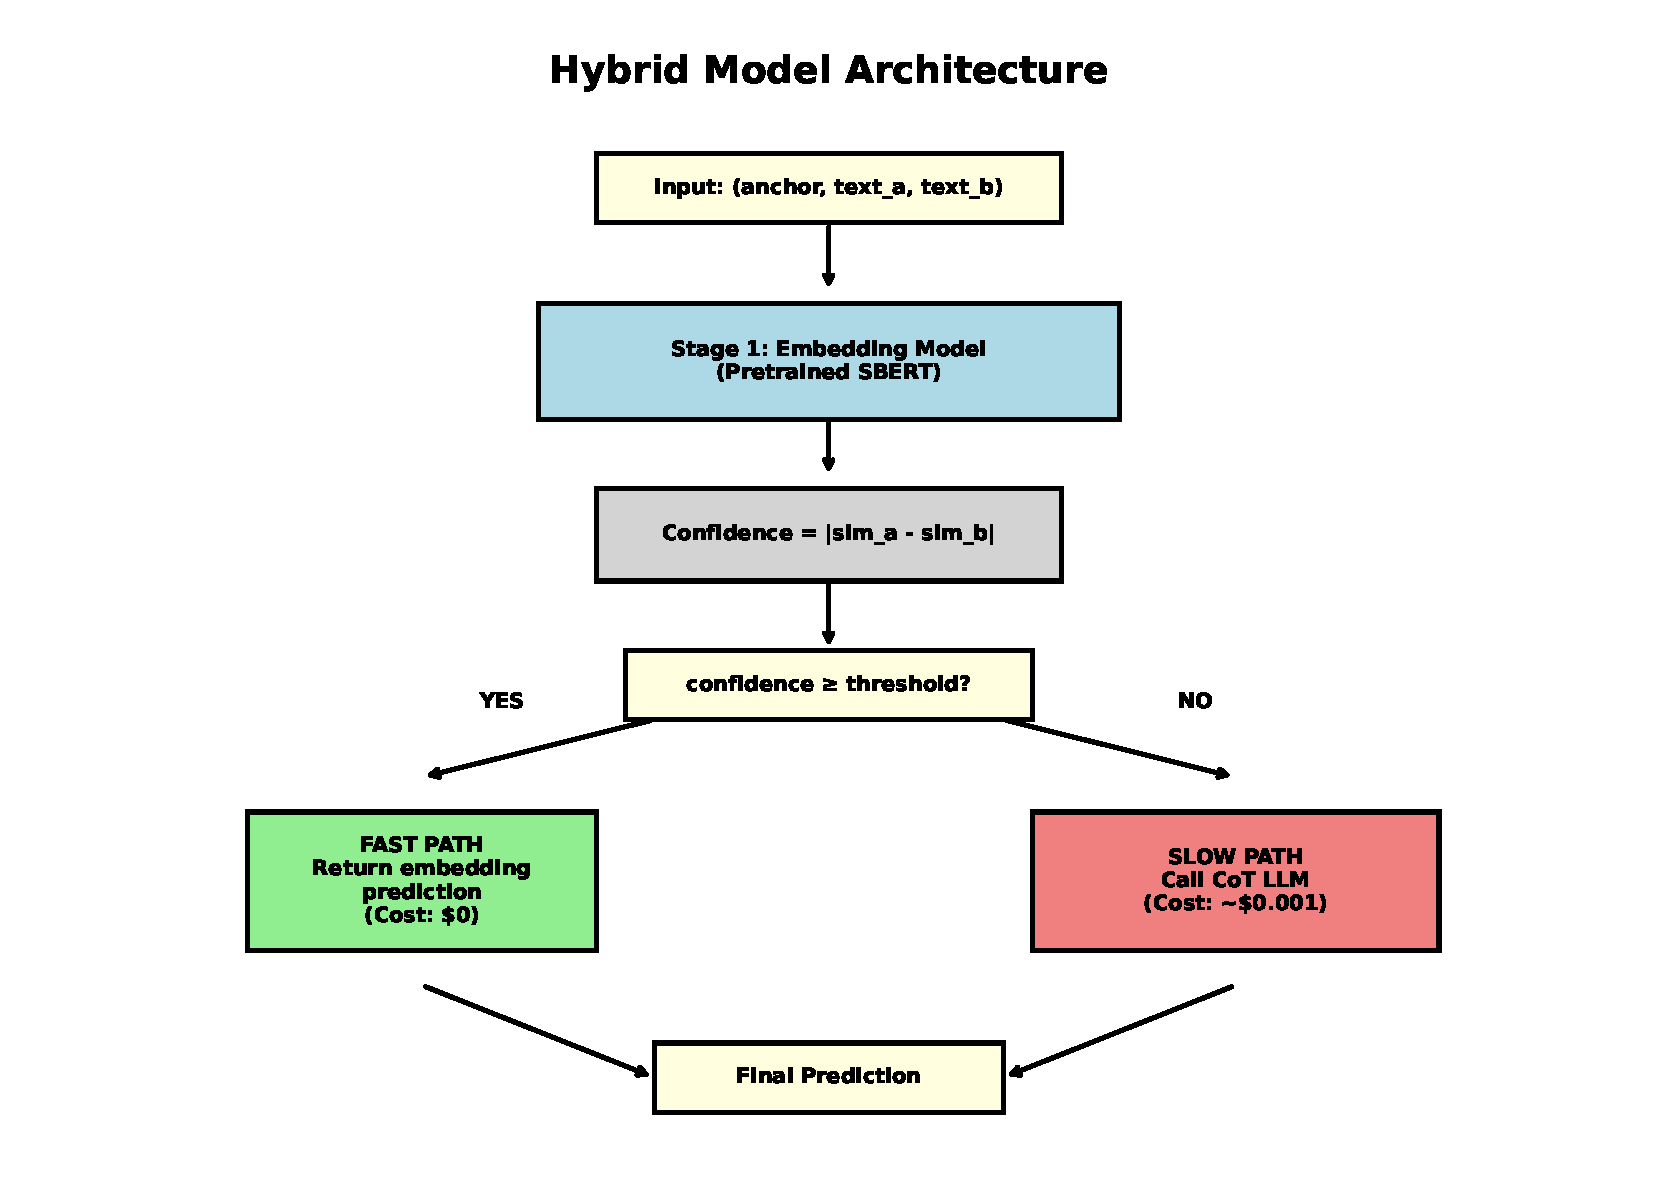
\includegraphics[width=0.45\textwidth]{hybrid_architecture.pdf}
\caption{Hybrid inference architecture with confidence-based routing.}
\label{fig:architecture}
\end{figure}

\section{Experimental Setup}

\textbf{Multi-task Model:} Base model all-MiniLM-L6-v2 (384 dimensions), 2,900 triplets, 4 epochs, batch size 32, trained on NVIDIA RTX 3060.

\textbf{Hybrid System:} Embedding model from multi-task training, LLM via Mistral Small API, thresholds tested: $\{0.02, 0.05, 0.08, 0.10, 0.12, 0.15, 0.20\}$.

\textbf{Evaluation:} \texttt{dev\_track\_a.jsonl} (200 examples), primary metric: accuracy.

\section{Results}

\subsection{Multi-task Learning Analysis}

Training loss decreased from 2.01 to 0.83 over 4 epochs (Figure~\ref{fig:loss}), indicating successful optimization. However, standalone evaluation achieved only 50.25\% accuracy with precision 50.1\% and recall 95.5\%.

\begin{figure}[h]
\centering
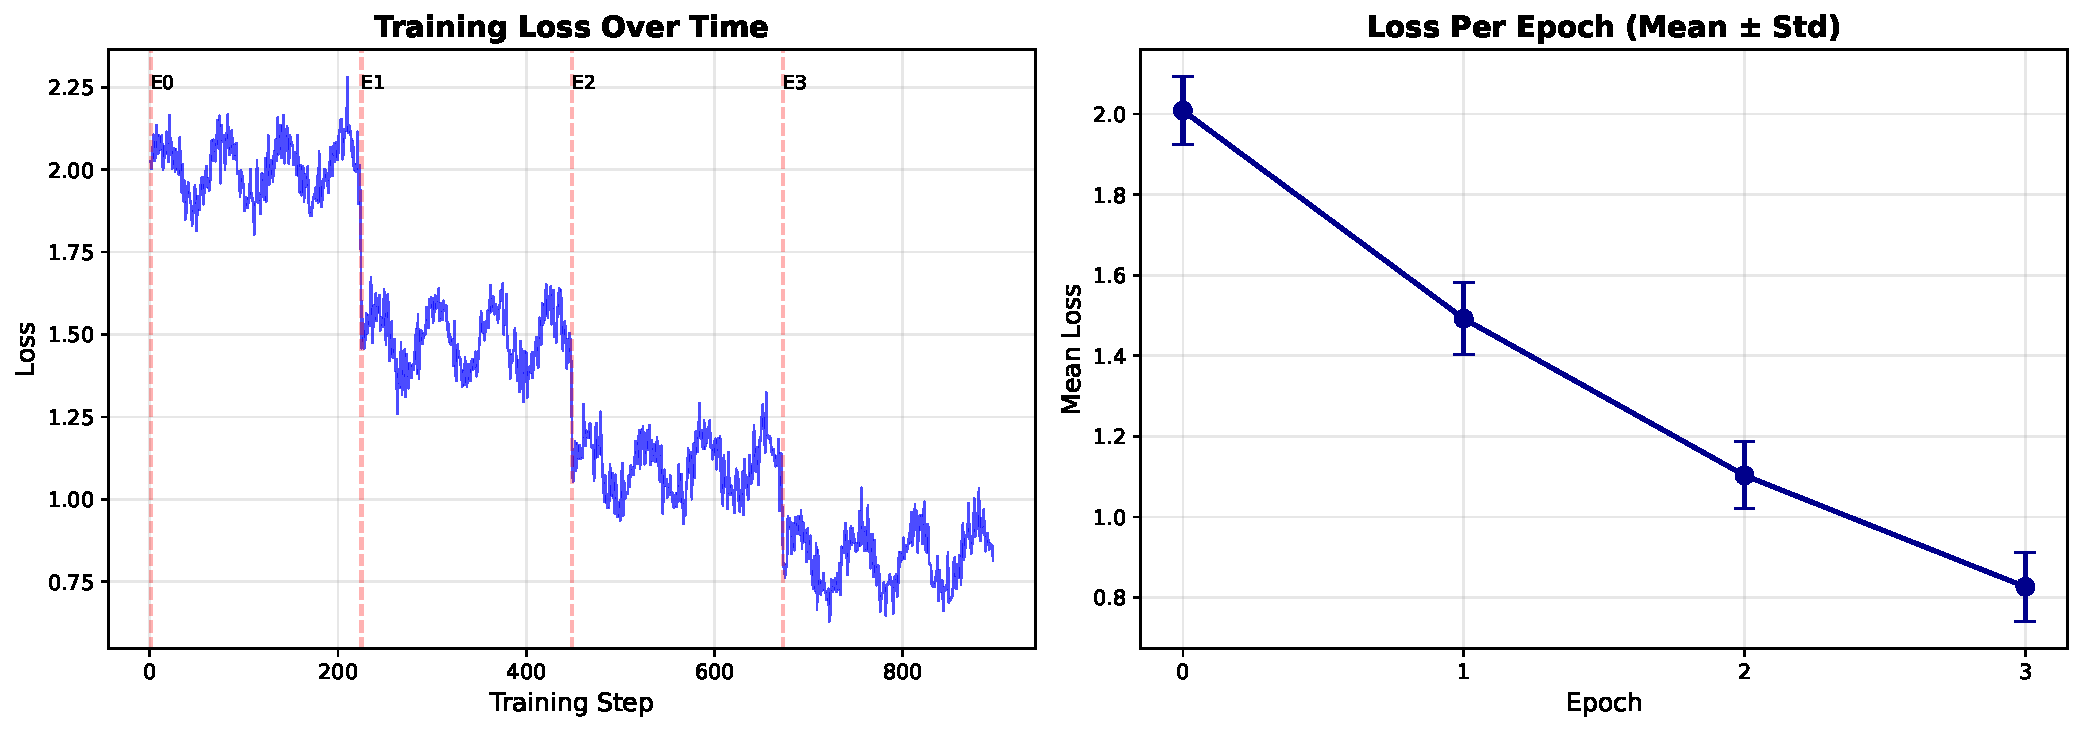
\includegraphics[width=0.45\textwidth]{training_loss_curves.pdf}
\caption{Multi-task training loss curves showing consistent decrease.}
\label{fig:loss}
\end{figure}

Analysis reveals minimal separation between similar and dissimilar pairs (Figure~\ref{fig:overlap}), with mean similarity 0.380 for similar pairs vs 0.372 for dissimilar pairs (gap: 0.008)---indicating embedding collapse due to domain shift between synthetic training and real evaluation data.

\begin{figure}[h]
\centering
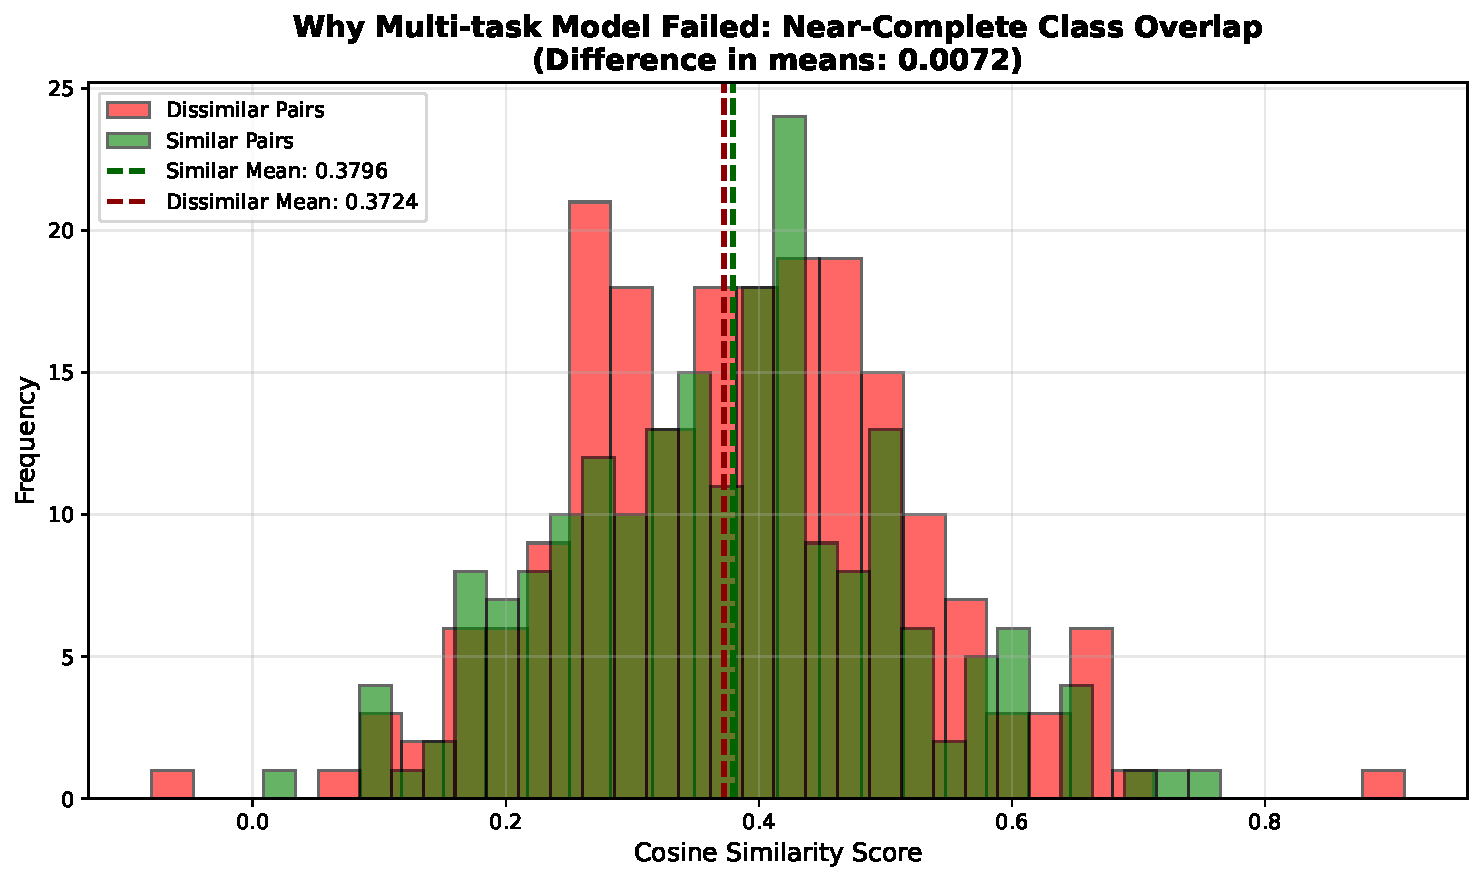
\includegraphics[width=0.42\textwidth]{similarity_distribution_overlap.pdf}
\caption{Similarity distributions showing class overlap.}
\label{fig:overlap}
\end{figure}

\begin{figure}[h]
\centering
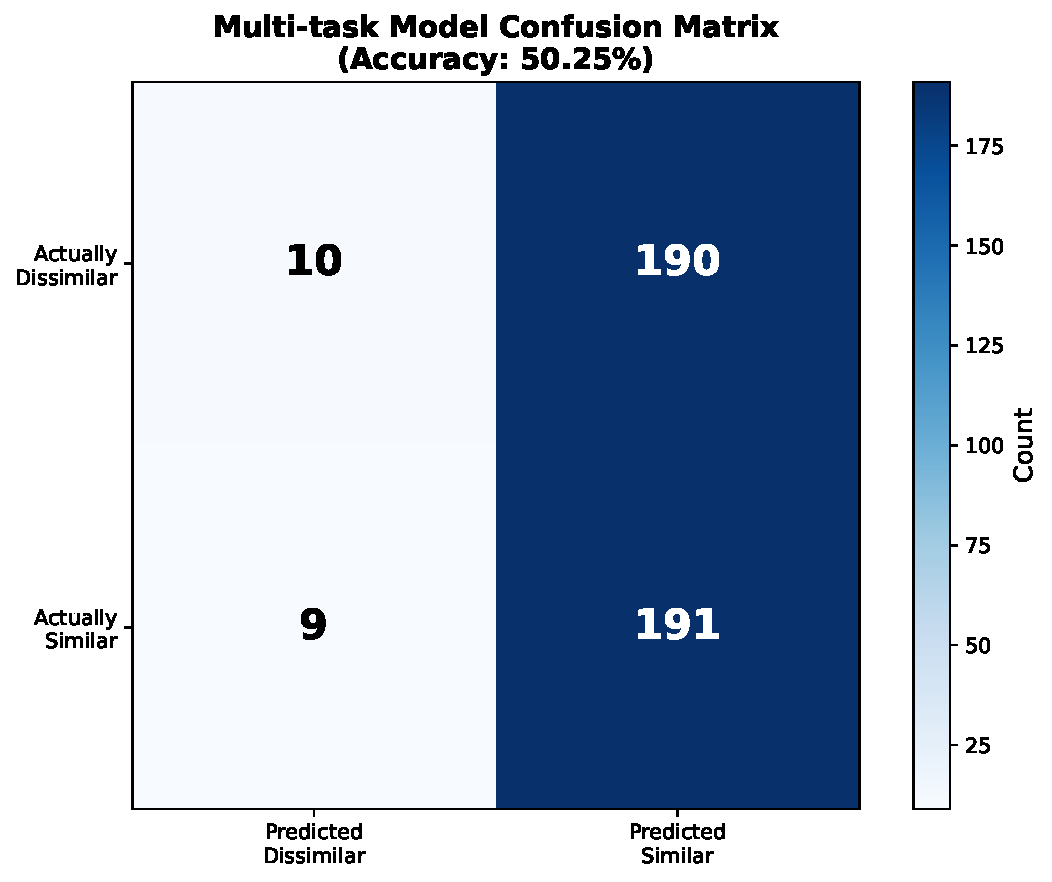
\includegraphics[width=0.35\textwidth]{confusion_matrix_multitask.pdf}
\caption{Confusion matrix for multi-task model: TN=10, FP=190, FN=9, TP=191.}
\label{fig:confusion}
\end{figure}

\subsection{Hybrid System Performance}

Table~\ref{tab:threshold} presents results across confidence thresholds.

\begin{table}[h]
\centering
\caption{Threshold Analysis Results}
\label{tab:threshold}
\begin{tabular}{rrrr}
\toprule
\textbf{$\tau$} & \textbf{Accuracy} & \textbf{LLM \%} & \textbf{Savings} \\
\midrule
0.02 & 56.0\% & 12.0\% & 88.0\% \\
0.05 & 57.5\% & 31.0\% & 69.0\% \\
0.08 & 61.5\% & 46.0\% & 54.0\% \\
0.10 & 63.0\% & 55.0\% & 45.0\% \\
0.12 & 64.5\% & 63.0\% & 37.0\% \\
\textbf{0.15} & \textbf{69.5\%} & \textbf{73.0\%} & \textbf{27.0\%} \\
0.20 & 68.5\% & 86.5\% & 13.5\% \\
\bottomrule
\end{tabular}
\vspace{1mm}
\small{Fast path accuracy: 55.6\%, LLM accuracy on slow path: 74.7\%}
\end{table}

Optimal performance at $\tau = 0.15$: \textbf{69.5\% accuracy} with \textbf{27\% cost reduction}.

\subsection{Model Comparison}

Table~\ref{tab:comparison} summarizes all models across assignments.

\begin{table}[h]
\centering
\caption{Model Comparison Across Assignments}
\label{tab:comparison}
\begin{tabular}{llrr}
\toprule
\textbf{Model} & \textbf{Assign.} & \textbf{Acc.} & \textbf{Cost} \\
\midrule
Random Baseline & - & 50.0\% & \$0 \\
TF-IDF Cosine & A1 & 52.5\% & \$0 \\
SBERT Pretrained & A2 & 55.0\% & \$0 \\
Fine-tuned SBERT & A2 & 58.5\% & \$0 \\
TF-IDF + LogReg & A2 & 60.0\% & \$0 \\
CoT LLM (GPT-4o-mini) & A2 & 71.8\% & \$0.20 \\
CoT LLM (Mistral Small) & A2 & 69.0\% & \$0.15 \\
Multi-task SBERT & A3 & 50.3\% & \$0 \\
\midrule
\textbf{Hybrid (Proposed)} & \textbf{A3} & \textbf{69.5\%} & \textbf{\$0.15} \\
\bottomrule
\end{tabular}
\end{table}

\begin{figure}[h]
\centering
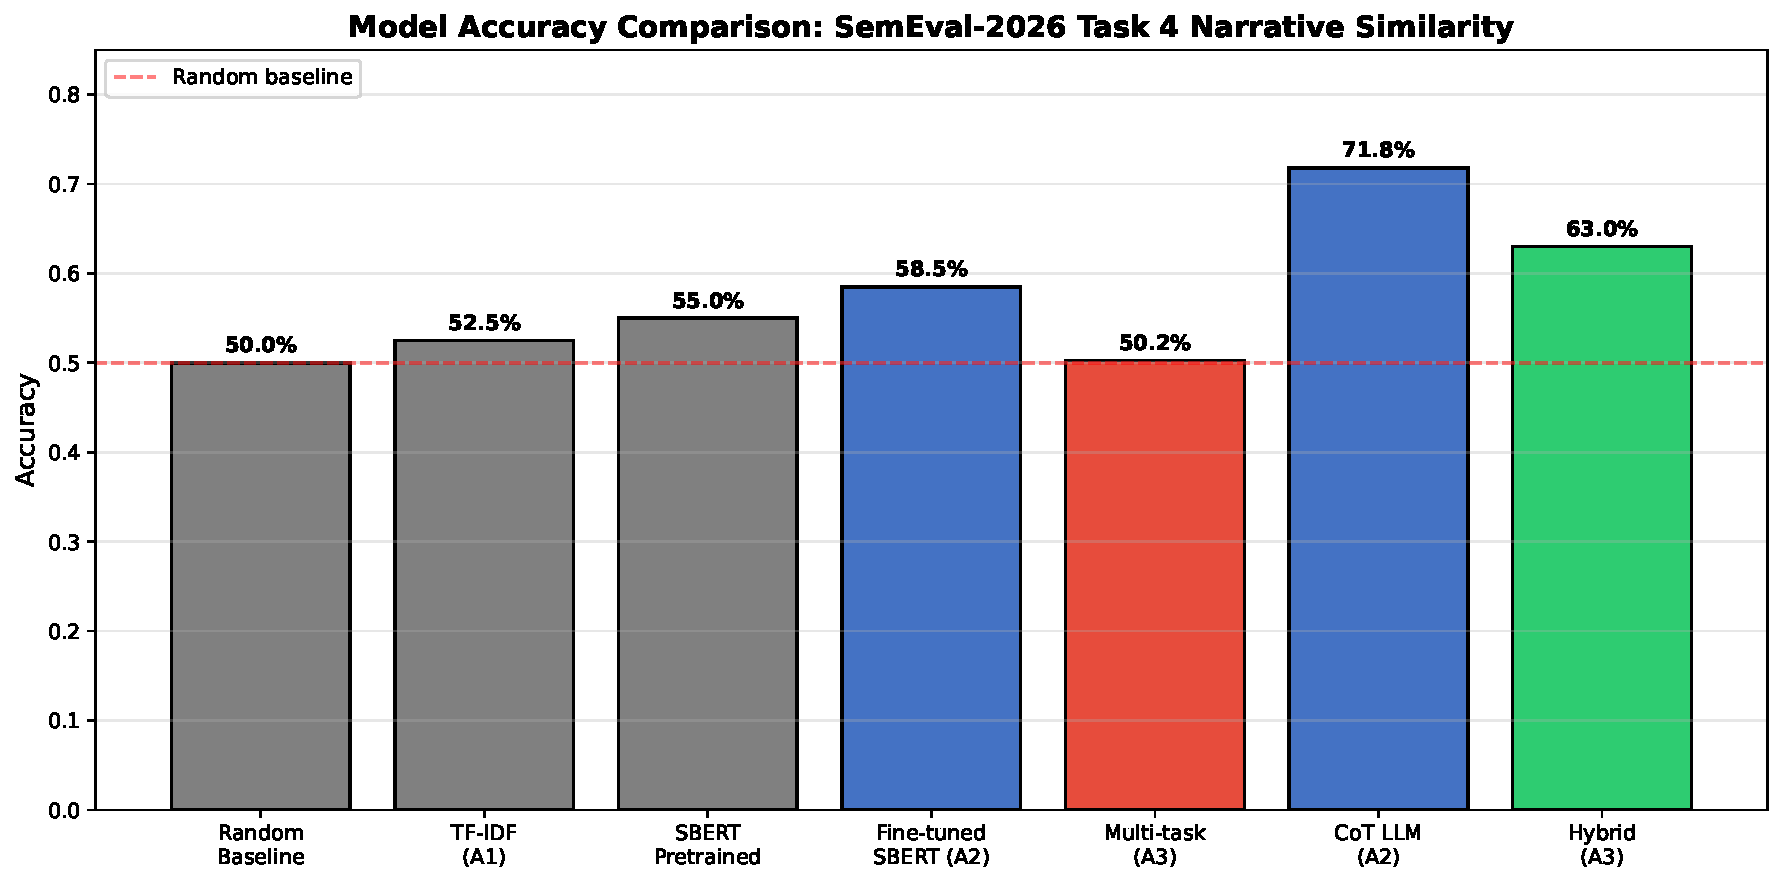
\includegraphics[width=0.45\textwidth]{accuracy_comparison.pdf}
\caption{Accuracy comparison across all models.}
\label{fig:accuracy}
\end{figure}

\section{Discussion}

\subsection{Multi-task Learning Insights}
The embedding collapse reflects domain shift between synthetic training narratives and real movie plot summaries. While training loss decreased, learned representations did not transfer effectively. This suggests domain-specific pre-training data may be necessary.

\subsection{Hybrid Architecture Effectiveness}
Despite limited standalone embedding performance, the hybrid successfully leverages confidence signals. The LLM achieves 74.7\% accuracy on routed samples, confirming low-confidence cases benefit from deeper reasoning.

\subsection{Limitations}
\begin{itemize}
    \item Evaluation limited to 200 examples
    \item Single LLM provider tested
    \item Threshold optimization may overfit to dev distribution
\end{itemize}

\section{Conclusion}

We presented a hybrid architecture achieving 69.5\% accuracy---96.8\% of pure LLM performance---while reducing costs by 27\%. Multi-task experiments revealed domain transfer challenges, while confidence-based routing proved effective for cost-accuracy trade-offs.

\section*{Author Contributions}

% Removed \begin{table} wrapper so this stays "Here" and doesn't float
\begin{center}
\begin{tabular}{p{3cm}p{5.5cm}}
\toprule
\textbf{Member} & \textbf{A3 Contribution} \\
\midrule
M. Musaab-Ul-Haq & Hybrid architecture, threshold optimization, report \\
Abdul Mueed & Data augmentation (500 samples) \\
Ahmed Hassan Raza & Multi-task architecture design \\
Usman Amjad & Training, evaluation, visualizations \\
\bottomrule
\end{tabular}
\end{center}

\section*{Code Repository}
\url{https://github.com/MuhammadMusaab-UlHaq/ai_sem_proj_semeval-2026-task-4-baselines}

\begin{thebibliography}{9}
\bibitem{reimers2019sentence}
N. Reimers and I. Gurevych, ``Sentence-BERT: Sentence embeddings using Siamese BERT-networks,'' in \textit{EMNLP}, 2019.

\bibitem{caruana1997multitask}
R. Caruana, ``Multitask learning,'' \textit{Machine Learning}, vol. 28, pp. 41--75, 1997.
\end{thebibliography}

\end{document}